\chapter{Introduction}\label{chap:intro}
\section{Von Neumann Architecture and the Memory Wall}\label{sec:memwall}
The field of computing is at a critical point. For decades, the industry has relied on the von Neumann architecture, which physically separates processing and memory units.
While incredibly successful, this paradigm has created an inherent "memory wall" \cite{gholami_ai_2024}, where the time and energy spent moving data between the CPU and memory now dominate the computation cost.
This bottleneck is especially evident in data-intensive fields like artificial intelligence and machine learning, which heavily rely on massive parallel operations, including  Matrix-Vector Multiplication (MVM) and Matrix-Matrix Multiplication (MM) \cite{gholami_ai_2024,khan_landscape_2024}.
As Moore's Law—which predicts that the number of transistors on a chip doubles approximately every two years, leading to exponential growth in computing power—slows down, simply shrinking transistors is no longer a sustainable path to improving performance.
This paradigm shift underscores the urgent need for innovative computing architectures capable of sustaining progress in computational efficiency and scalability.

\section{Dissertation Objective and Motivation}\label{sec:obj}

The "memory wall" has motivated a global research effort focused on new computing paradigms that move beyond the traditional von Neumann architecture.
Among the most promising is Computing Near-Memory (CNM) and Computing In-Memory (CIM) \picref{fig:cim}, the idea of which is to perform computation directly where data is stored, eliminating the costs of data movement \cite{khan_landscape_2024}.
Among the CIM branches, Phase-Change Memory (PCM) has emerged as a possible candidate to enable Analog In-Memory Computing (AIMC) as its analog resistance states can naturally represent the weights of a neural network, and the way the crossbar is configured allows for efficient analog and parallel computation.

However, designing and fabricating new hardware accelerators is a high-risk, high-capital process. 
Before committing to silicon, it is essential to have robust virtual platforms to explore architectural trade-offs, 
validate functionality, and co-design the necessary software. This project is motivated by the need for such a virtual prototype.

The primary objective of this dissertation is to implement and validate a virtual prototype of a PCM-based AIMC accelerator within the GVSoC \cite{bruschi_gvsoc_2021} simulator for the Parallel Ultra-Low-Power (PULP) platform.
PULP is an open-source hardware and software framework based on the RISC-V instruction set architecture (ISA), which aims to provide low-power computing systems.

To achieve this objective, two main goals were established:
\begin{itemize}
\item Develop a C++ model of a PCM accelerator capable of performing MVM operations, integrated as a memory-mapped peripheral in GVSoC.\\
\item Investigate and implement performance optimisations for the simulation model to enable efficient and fast simulation even on limited hardware resources.
\end{itemize}

\begin{figure}[H]
  \centering
  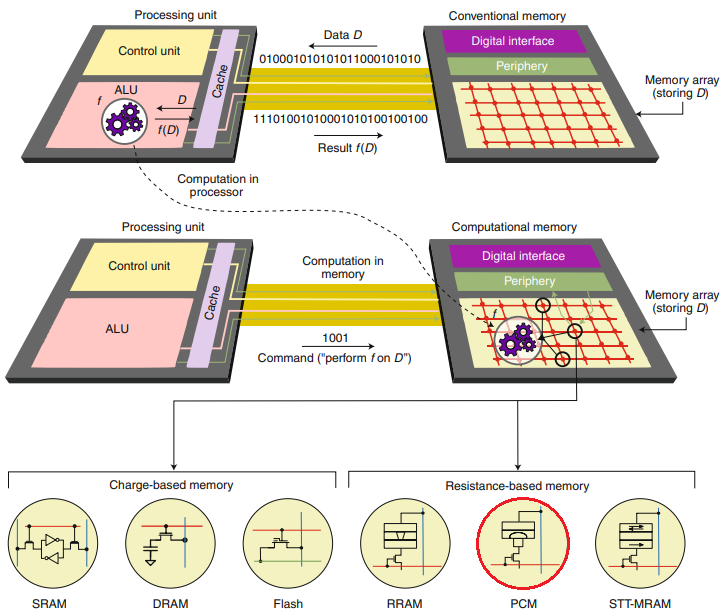
\includegraphics[width=0.8\textwidth]{Figures/CIM.png}
  \caption{Computing In-Memory (CIM) architecture overview, moving computation closer to memory to alleviate the von Neumann bottleneck. Adapted from \cite{sebastian_memory_2020}.}
  \label{fig:cim}
\end{figure}

\section{Summary of Contributions}\label{sec:contri}
This dissertation makes several contributions to the field of hardware acceleration and virtual prototyping for next-generation computing architectures.
The primary outcomes of this research are the following:
\begin{itemize}
\item \emph{A configurable virtual prototype of a PCM accelerator}.
The core contribution is a fully functional C++ model of a PCM-based AIMC accelerator integrated into the GVSoC framework.
This model is not just an abstract component but a working, configurable, peripheral that can be simulated within a complete System-on-Chip 
environment, serving as a valuable tool for architectural exploration.\\
\item \emph{Demonstration and analysis of simulation optimisation techniques}.
This work demonstrates the effectiveness of applying advanced software optimisation principles to hardware simulation.
By implementing and benchmarking techniques such as flattened data buffers and multithreading, this project offers a strategy for significantly enhancing the performance and scalability of virtual prototyping, allowing for large-scale experiments even on platforms with limited computational resources.
\end{itemize}
